\documentclass{beamer}
\usetheme{Madrid}

% escreve textos gerados em portugues
\usepackage[brazilian]{babel}
% aceita unicode
\usepackage[utf8]{inputenc}

\author[Andre Esteve and Zhenlei Ji]{
Andre Petris Esteve - \texttt{andreesteve@gmail.com}\\
Zhenlei Ji - \texttt{zhenlei.ji@gmail.com}}
\institute[IC\textbackslash UNICAMP]{
MC806 - Operational System Topics\\}

\title[Linux VFS]{Linux Virtual File System}
\subtitle[]{The linux VFS and FUSE - File System in User Space}

\date[10/20/2011]{October 20th, 2011}

\begin{document}

%--- create section frame for every new section --%
\AtBeginSection[]
{
   \begin{frame}
       \frametitle{Agenda}
       \tableofcontents[currentsection]
   \end{frame}
}

\begin{frame}[plain]
  \titlepage
\end{frame}

%--- content -------------------------------------%
\begin{frame}{Agenda}
  \tableofcontents
\end{frame}

\section{Objectives}

\begin{frame}{Objectives}

  \begin{block}{What do we want?}

	\begin{itemize}

		\item{View the Linux's Virtual File System as a series of object oriented entities (classes and objects)}

		\item{Construct UML models to easy understanding}
		
		\item{Provide initial information so one can start developing a file system module for the Linux kernel}
	
	\end{itemize}

  \end{block}

\end{frame}

\section{Linux's Virtual File System Overview}

\begin{frame}{What's Linux's Virtual File System}

  \begin{block}{Definition}

	The Virtual File System (also known as the Virtual Filesystem Switch)
	is the software layer in the kernel that provides the filesystem
	interface to userspace programs. It also provides an abstraction
	within the kernel which allows different filesystem implementations to
	coexist. \footnotemark

  \end{block}

	\footnotetext[1]{Overview of the Linux Virtual File System, Richard Gooch, from Linux "documentation"}

\end{frame}

\begin{frame}{Linux's Virtual File System Overview}

	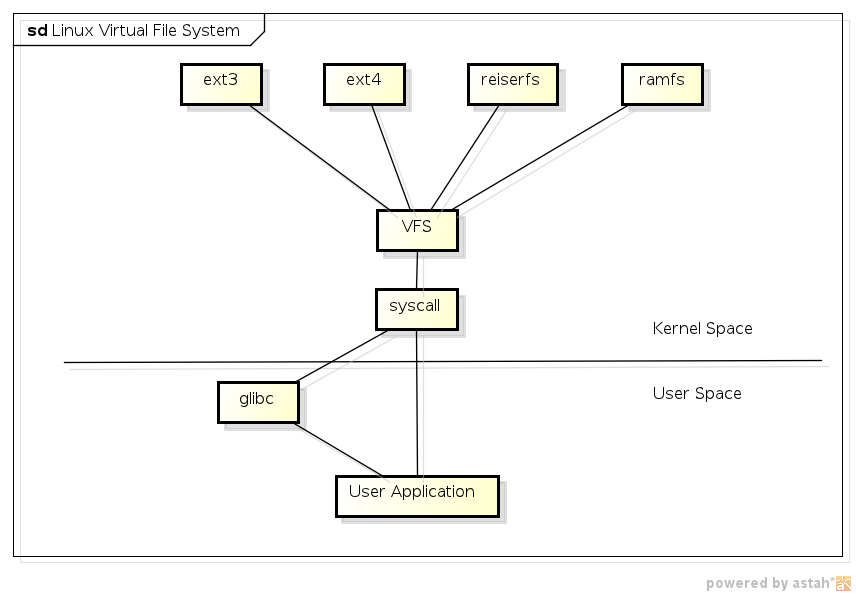
\includegraphics[scale=0.5]{img/vfs_overview.png}

\end{frame}

\begin{frame}{Linux's Virtual File System Overview}

	\begin{itemize}
	
		\item[$\bullet$]{Abstraction layer to allow different fs\footnotemark[1] to coexist}	
		\item[$\bullet$]{Only point of access to fs calls}
		\item[$\bullet$]{Implements common fs operations}
			\begin{itemize}			
				\item[$-$]{Common inicialization operations}
				\item[$-$]{Mounting (at a certain level) and managing mount points}
				\item[$-$]{Path lookup}
				\item[$-$]{Caching}
			\end{itemize}	
	\end{itemize}

	\footnotetext[1]{Shot for "file system"}

\end{frame}

\begin{frame}{Linux's Virtual File System Overview}

	\begin{block}{How is a file system implemented?}
		With loadable kernel modules\footnotemark[1] (LKM), or just modules for short.
	\end{block}

	\vspace{15pt}

	\begin{itemize}
	
		\item[$\bullet$]{It's possible to compile a LKM with the base kernel}
		\item[$\bullet$]{Or just load the LKM during system usage}

	\end{itemize}

	\footnotetext[1]{For an extensive discussion about LKM, see: \texttt{http://www.tldp.org/HOWTO/Module-HOWTO/}}

\end{frame}

\section{Linux's Virtual File System Core Elements}

\begin{frame}{Linux's Virtual File System Core Elements}

	\begin{description}\itemsep4pt
			
		\item[vfsmount]{Mount point information}
		\item[file\_system\_type]{Information about a specific fs type}
		\item[super\_block]{Represents a mounted file system}
		\item[inode]{Information about a file (on disk, memory or network)}
		\item[dentry]{A directory entry}
		\item[file]{A file abstraction - points to a inode}

	\end{description}

\end{frame}

\begin{frame}{Linux's Virtual File System Core Elements}
	
	\center{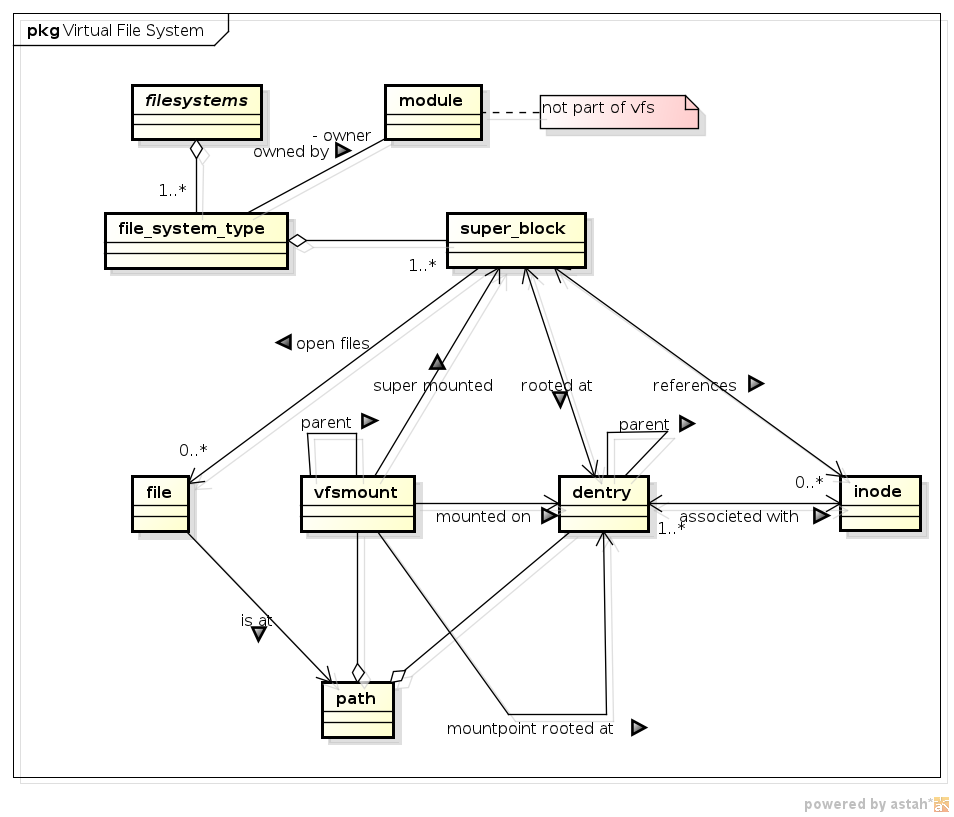
\includegraphics[scale=0.35]{img/vfs_elements_simple.png}}

\end{frame}

\subsection{file\_system\_type}

\subsection{vfsmount}

\subsection{super\_block}

\subsection{inode}

\subsection{dentry}

\subsection{file}


%--- obrigado-------------------------------------%

\begin{frame}[plain]

  \begin{center}
    \Huge Questions?
  \end{center}

  \vspace{0.2in}

  \begin{center}
	Andre Petris Esteve - \texttt{andreesteve@gmail.com}\\
	Zhenlei Ji - \texttt{zhenlei.ji@gmail.com}
  \end{center}
\end{frame}

\end{document}
